\section{Methodology}
\label{sec:researchDesign}

In the following subsections, we discuss data collection and analysis for the performed studies. For naming the studies, we follow the terminology for Software Engineering research strategies from Stol and Fitzgerald~\cite{Stol2015}: an experimental simulation (Section~\ref{sec:expPart}), a judgment survey (Section~\ref{sec:surveyPart}) and a case study (Section~\ref{sec:caseStudy}). The package for these studies is available online~\cite{package-bib}.

\subsection{Experimental Simulation}
\label{sec:experiment}

%GQM
In this study, we investigate the use of
public contracts in simulated programming tasks, concerning effectiveness and understandability, from the point of view of Java developers.

\subsubsection{Participants}
\label{sec:expPart}

%recruitment
We selected participants among professional developers assigned to projects in the context of a major R\&D Institute in Brazil. Recruitment was carried out by invitation; from estimated 150 invited professionals, 24 of them accepted and later received the assignment material by e-mail. The only requirement was previous experience with Java. From the 24 recruited developers, 10 of them had computer science (or related) degrees, while the remaining were carrying out undergraduate studies in the field. 
%number of participants
Although the number of participants is small for generalising any conclusions, we expect the observations to be considered as an exploratory model to be checked by future studies with larger samples. For experimental simulations, our participant set is within the expected size~\cite{Stol2015}.


\subsubsection{Study Design}
\label{sec:studyDesign}

%factors
The study was designed to assess the effect of a given contract style on implementation tasks which depend on documented APIs. 
%factor 1
Participants were assigned to use a contract style (Factor 1) from the following: \emph{Textual Javadoc, \contractjdoc{} and JML-like formal contracts}. Table~\ref{tab:factorsEmpStudy} displays the treatments for those two factors.
%factor 2
For each of those styles, two kinds of task are considered (Factor 2): a \textit{Supplier} task, in which the participant must program the implementation of a Java API, and a \textit{Client} task, which demands development of client code for the API.
%factor 3
An additional variation we included regards the particular API assigned to an arbitrary participant (Factor 3): \textit{Stack} or \textit{Queue}. We chose to use simple and well-known interfaces trying to avoid the confounding effect that lack of knowledge could bring to the study.


\begin{table}[ht]
\caption{Factors and treatments of the empirical study.}
\label{tab:factorsEmpStudy}
\centering
\begin{tabular}{ll} \toprule
\bfseries Factors & \bfseries Treatments \\
\hline

\multirow{3}{*}{\textbf{Approach}} & \contractjdoc{} \\
 & Textual Javadoc \\
& JML-like formal contracts \\ \hline 
\multirow{2}{*}{\textbf{Task}} & Client \\
& Supplier \\ 
\bottomrule
\end{tabular}
\end{table}

%design
We use a factorial design~\cite{wohlin}, randomly assigning participants to each combination of treatments; a trial is the triple $<style, task, API>$.
Since there are three contract styles, two types of task and two APIs, there are 12 possible trials, so each of them was carried out by two participants, resulting in a balanced design. 
The assignment of participants was random, to minimise bias.

\subsubsection{Experimental Procedure}
\label{sec:expProcedure}

The experiment was performed offline, i.e., participants received the experimental package via an online survey platform that we use to collect the results.
% double blind process 
% An example of survey sent to the
% participants can be found online.\footnote{\url{https://goo.gl/forms/ySTsYfKSRcotLayk1}} 
The experimental package consisted of \emph{(i) a statement of consent, (ii) a pre-test
questionnaire, (iii) instructions and materials to perform the experiment, and (iv) a post-test questionnaire}. 
The instructions contained what we expected from the participants: they were asked to perform an implementation task (a supplier or a client code) for the
provided API. Each participant received one of the following tasks: create a class that implements the API, or a client code using the API's methods.
We also asked each participant to fulfil a pre-study questionnaire reporting their programming experience (concerning Java and contract-based programming experience). 
%After filling in the questionnaire, we randomly assign a task.

During the assignment, participants were allowed to review additional information -- part of the experimental package -- about the assigned contract style. 
%the tasks 1
For \textit{Supplier} tasks, participants should have implemented variations of well-known stack (or queue) operations whose intended behaviour was documented using one of the three contract styles. The following example shows the contract for \lstinline!Queue.add!, written in textual Javadoc:

%example
\begin{lstlisting}[basicstyle=\footnotesize\ttfamily,name=figxpi, frame=lines, mathescape=true]
/**
   * Inserts the specified account into the queue 
   * if it is possible to do so 
   * immediately without violating capacity 
   * restrictions, returning true upon 
   * success and throwing an AccountQueueException 
   * if no space is currently available.
   * @param acc - the account to be added. 
   *     Must not be null.
   * @return true if the operation occurs with success.
   * @throws AccountQueueException - if the queue is 
   *     full or the account is null.
   */
  public boolean add(Account acc) throws AccountQueueException;
\end{lstlisting}

%the tasks 2
Differently, \textit{Client} tasks were carried out based on textual descriptions, although any call to API should fulfil its external contracts, also presented using one of the three documentation options. Implementation of the API was provided as binaries, so participants were not given access to the source code.
%post-study
Before submitting the programs, we asked the participants to answer a \emph{post-experiment questionnaire}, in which we collected qualitative information about the developers' view of each task.

We performed a pilot with three developers in order to adjust the questionnaires' structure.
%the way in which we make the data available for the developers. 
As a result, we changed the way of making the artefacts available to participants. 
At first, we were making the documented interface available in a link and the working dataset in another. 
Pilot participants highlighted this, indicating that a single package containing all Java classes should be located in a single URL.

\subsubsection{Research Method}
\label{sec:labmethod}

%method for checking correctness
Each program sent by the participants were subjected to a test suite especially implemented by the researchers for checking whether every single contract was fulfilled -- \emph{there was a test case for each contract clause}.
As a result, we can classify each submission according to the number of faults detected by these tests.
%method for Likert
To analyse the understandability assessments in the post-study questionnaire, we applied simple visualisation techniques (boxplots and bar charts) and statistical tests; in this case, we used the \emph{Wilcoxon rank sum test}~\cite{statistical} for testing difference between groups, with non-normal data.

%method for analysing questionnaire info
The answers from the qualitative post-study questionnaire were subject to a simple content analysis, performed by two researchers, which held a joint session for agreement on the category for each response from the developers. 
 We used \emph{open coding}~\cite{Price2010} to analyse the collected answers, by inspecting them quote by quote and detecting categories, representing the key ideas in the data.




\subsection{Judgment Survey}
\label{sec:survey}

%goal, question, metric
The goal of the survey is to compare three contract styles (Javadoc text, \contractjdoc{} and formal contracts) concerning understandability, from the point of view of Java developers. 

\subsubsection{Participants}
\label{sec:surveyPart}

%who to survey - convenience sample
We selected participants utilising a non-probability convenience sample~\cite{wohlin}. 
The survey link was sent to academic and professional mailing lists.
%snowball approach - contacts
Also, our contacts were asked to follow a snowball approach, sending the survey to their respective
contact lists, increasing the sample and the number of participants in our study.
%number
The survey was open for three weeks (from June to July 2016) and received 142
answers (from an estimated total of 700 contacts who were sent the link -- approximately a 20\% response
rate). From the 142 participants, 51 (36\%) are professionals, and 91 are computer science students.


\subsubsection{Design and Method}
\label{sec:surveyDes}

%survey method
For this study, we followed a quantitative method based on a web-based survey instrument, suited to measure opinions and behaviours in response to specific questions~\cite{refSurvey}, in a non-threatening way. 
%web-based survey
% double-blind
% The questions were available as an online form\footnote{http://goo.gl/forms/XcEqvPH0Eq920jaA3}. 
%survey structure
The survey
instrument
%\footnote{\url{https://goo.gl/forms/8W9jUMGCavkkzDj12}} 
begins with a purpose of clarification along with a consent term.
Then, a characterisation of the respondent is given by questions related to Java experience and experience with contract-based programming. Next, the survey is presented: links for three Java interfaces with each one documented in a different approach is shown, then some questions related to the understanding of the behaviour of a class implementing the interfaces based on the comments available is asked. 

%likert scale
We applied \emph{Likert-scale} questions. In two questions we ask the developers to choose the most understandable documentation approach: one specific -- related to the provided contract style; and one general, concerning the use of the approach in a general context.
%pilot study
We also conducted a pilot concerning the questions and the structure of the programs being used. The pilot consists in asking three Java developers to test the setup for the survey, allowing us to adjust the survey's questions and structure. The developers who participated, however, did not report issues on the structure that we used for presenting the needed data for the participation in the study.

%methods
Regarding quantitative methods, we applied \emph{Wilcoxon, and Kruskal-Wallis rank sum tests}~\cite{statistical} for comparing the results for the different groups of participants. Regarding survey results, we applied \emph{one-way analysis of variance (ANOVA), Tukey HSD} and pairwise comparisons using \emph{t-tests with Bonferroni correction}~\cite{statistical}.%in addition, we employed Wilcoxon rank sum test with continuity correction tests.

\subsection{Case Study}
\label{sec:caseStudy}
%goal
This study aims at assessing the usefulness of contract expressions within Javadoc text, concerning automation benefits, from the point of view of Java developers. 
%metric
%We observe the results from applying adding contract expressions to \totalSystems{} real, Javadoc-rich open source systems; all their method-level Javadoc annotations are manually translated to contract expressions, before running tests looking for mismatches between specifications and actual method behaviour.

\subsubsection{Systems Selection} 
\label{sec:systems}

%which systems
The case study was performed on a convenience sample: \totalSystems{} Javadoc-rich open source systems available at GitHub\footnote{\url{https://github.com/}} repository.
%criteria
The selected systems presented the highest rate of method-level Javadoc commentary including the following set of key phrases: \emph{``must be'', ``must not be'', ``should
be'', ``should not be'', ``greater than'', ``not be null'', ``less than''}.
After some visual filtering, we collected the five most important classes in
each system, based on overall dependence, and check whether those classes
contained method-level Javadoc comments for most of their methods. If so, the
system is selected. Finally, we checked whether the system presented a test suite, which is run during the case study to detect anomalies. We
were able to find five systems meeting these criteria.
%system descriptions
See Table~\ref{tab:Units} for details about the selected systems. 

%While \texttt{ABC-Music-Player}\footnote{\url{https://github.com/deepakn94/ABC-Music-Player}} plays music from an ABC file (part of a project assignment from MIT class 6.005), \texttt{Dishevelled}\footnote{\url{https://github.com/heuermh/dishevelled}} hosts free and Open Source libraries for several user interface components and supporting code, with emphasis on views and editors for complex data structures, like collections, sets, lists, maps, graphs, and matrices; \texttt{Jenerics}\footnote{\url{https://github.com/mriedel/Jenerics}} is a general-purpose set of Java tools and templates library. On the other hand, \texttt{OOP Aufgabe3}\footnote{\url{https://github.com/rwilli/aufgabe3}} aims to manipulate polygons. In addition, \texttt{Webprot\'{e}g\'{e}}\footnote{\url{https://github.com/protegeproject/webprotege}} is a collaborative ontology development environment for the Web. Those systems amount to more than 190 KLOC. 

%total contract clauses (\#CC) we were able to write
%-- following \cite{Estler-etal14} approach, in which the number of contract clauses is a proxy for contract complexity -- 
%as split into pre-conditions (\#Pre) and post-conditions (\#Post).\footnote{The clauses correspond to the contracts we applied in each system.}

%systems table
\begin{table}[ht]
\caption{Case study Systems. LOC shows the code lines (LOC), total contract clauses (\#CC) and a brief description.}
\label{tab:Units}
\centering
\begin{tabular}{lrl}
\toprule
\bfseries System &  \bfseries LOC & 
\bfseries Description  \\ \hline
ABC-Music-Player & 1,973 & Music player from ABC files  \\ 
Dishevelled & 110,577 & UI components for complex data structures.\\ 
Jenerics & 2,538 &  General-purpose set of Java tools and templates.\\ 
OOP Aufgabe3 & 353 &  Routines for polygon manipulation.\\
Webprot\'{e}g\'{e} & 74,742 & Environment for ontology development. \\ \hline

 \bfseries Total &  \bfseries \totalCode{} & \\
\bottomrule
\end{tabular}
\end{table}

%what is pre-condition, post-condition and invariant in Javadoc
%criterio para a traducao
The manual translation abides by the following criteria: method-level comments were considered pre-conditions
if the comments establish some restriction over the method parameters.
For instance, \texttt{``@param notes - Should not be null and should be of length >= 2''} was
replaced by the following \contractjdoc{}-based expression \texttt{[notes != null \&\& notes.size() >= 2]}, and
post-conditions that establish details on the return value of the
methods, e.g. \texttt{``@return Integer the number of edges. Is always >= 3''}
was replaced by \texttt{[@return >= 3]}. 
%$Class-level comments make up for invariants when they describe properties over fields that must be maintained for all methods of the class.

\subsubsection{Experimental Procedure and Research Method} 

%tasks
%translation
Three researchers applied \contractjdoc{} in \totalSystems{} existing open-source systems
available at GitHub (Table~\ref{tab:Units}). They followed a bottom-up approach for
writing the \contractjdoc{} contracts: the researchers started applying
\contractjdoc{} in the simplest methods and classes (or interfaces), following
up to the most complex. Contracts followed the Javadoc comments available in
natural language (in English).
%and some of them were inferred from the methods' source code.
%As result, they wrote \totalClauses{} contract clauses: \totalPre{} pre-conditions and \totalPost{} post-conditions.
% and \totalInv{} invariants (see
Figure~\ref{fig:applicationProcess} presents the steps performed by the researchers when applying
\contractjdoc{} to the systems. The process is composed of four steps: 1) generation of the
contracts based on the natural language comments available (as shown in
Section~\ref{sec:systems}); 2) compilation of the contracts by means of
\contractjdocCompiler{} compiler, to generate the bytecode enriched with assertions; 3) the test suite available in each system is run over the contract-aware bytecode; 4) results of the test suite execution are analysed and
anomalies are investigated.

\begin{figure}[h]
\centering
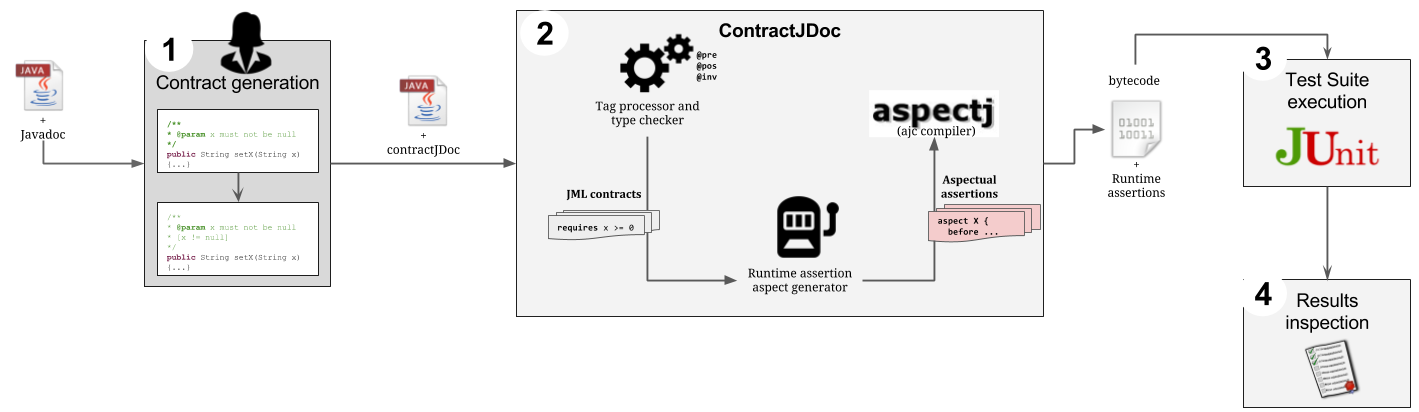
\includegraphics[width=1.0\textwidth]{figs/ContractJDocProcess}
\caption{Steps for applying \contractjdoc{} to Javadoc-annotated systems.}
\label{fig:applicationProcess}
\end{figure}

%contract classification
We group the contracts according to
the approach introduced by Schiller et al.~\cite{typeContracts}: application-specific contracts, which enforce richer semantic properties;
common-case contracts, which enforce
expected (common) program properties;
and code-repetitive contracts, which repeat exact statements from the code.

%experiment package - link
All systems used in this study are available in a replication
package.\footnote{\url{https://goo.gl/yO8or2}; in order to run the
\contractjdoc{} compiler, the folder \textit{aspectjml-lib} must be copied into the folder of each system.}
%when we consider an error
Concerning the verification performed after applying \contractjdoc{} contracts into the systems,
we used the test suites available with the purpose of identifying problems
(four systems include a test suite).
Every test case that failed prompted for further investigation for confirming the presence of an anomaly.

% applying dbcjdoc
As a secondary goal, the study allowed us to check the expressiveness of \contractjdoc{} and to
evaluate the effort related to adding contracts to existing systems.
Besides, we enhanced the compiler and added features to simplify
the process of applying \contractjdoc{} in existing projects.

